\documentclass[aps,prd,10pt,onecolumn,nofootinbib,superscriptaddress,floatfix]{revtex4-2}

\usepackage[T1]{fontenc}
\usepackage{lmodern}
\usepackage[utf8]{inputenc}
\input{glyphtounicode}
\pdfgentounicode=1
\usepackage{amsmath,amssymb,mathtools}
\usepackage{bm}
\usepackage{graphicx}
\usepackage{placeins}
\usepackage{hyperref}

\hypersetup{
  colorlinks=true,
  linkcolor=blue,
  citecolor=blue,
  urlcolor=blue
}

\begin{document}
\raggedbottom

\title{Can a Wormhole Induce a Monopole?}

\author{Sergei Slobodov}
\email{sergei@slobodov.com}
\noaffiliation

\date{\today}

\begin{abstract}
Could a body orbiting near one mouth of a traversable wormhole make the mass
seen near the other mouth rise and fall?  We show that the local vacuum
Einstein equations keep the first-order mass monopole constant on a
Schwarzschild background, even for nonspherical source motion.
Beyond first order, the Bondi mass at an observer end that is vacuum near future
null infinity cannot increase, even with an evolving throat.  For mouths
sharing one exterior, this result is recovered in an assumed regular
two-ended limit as their separation grows.
Source motion can nevertheless modulate radiative mass loss.
The Maxwell counterpart is exact: without current crossing the measuring
surface, the measured monopole charge remains constant.
The local gravitational and Maxwell results require neither a compact
interior nor an asymptotic end.
\end{abstract}

\maketitle

\section{Introduction}
\label{sec:introduction}

A wormhole can support a static mass at either mouth.  Dai and Stojkovic
(DS) propose that a body orbiting near one mouth makes the mass seen near
the other rise and fall \cite{DaiStojkovic2019Observing}.

In the DS model, two Schwarzschild exteriors are joined at throat radius
$R$, with a mass $\mu$ at radius $A$ in one exterior.  Replacing $A$ by
$A(t)$ in the static observer-side field produces the periodically
varying $1/r^2$ acceleration also used by
Simonetti et al.~\cite{SimonettiEtAl2021SensitiveSearches} and
Moiseev and Sazhina~\cite{MoiseevSazhina2025ObservationalSearch}.

A family of static solutions need not describe an allowed evolution.
We show that Maxwell charge is exactly conserved without current through
the measuring surface.  In gravity, the first-order mass monopole is
constant in a Schwarzschild vacuum region.  Both results are local and
require neither a compact interior
nor an asymptotic end.

Beyond first order, we use the exact Bondi mass-loss law.  When the observer
end is vacuum near future null infinity, its mass can decrease through
radiation but cannot rise and fall periodically, even with an evolving
throat.  For mouths sharing one exterior, this result is recovered in an
assumed regular two-ended limit as their separation grows.  These
asymptotic results require no small-source approximation.

Appendix~\ref{app:quadrupole} gives a quasistatic quadrupole benchmark.
We use $G=c=1$ and $r_g=2M$, where $M$ is the background Schwarzschild
mass; only the local Schwarzschild calculation and benchmark assume
$\mu/M\ll1$.

\section{Conservation of electric monopole charge}
\label{sec:maxwell}

In the DS electrostatic model, two flat exteriors are joined at $r=R$,
with charge $q$ at $r_1=A$ in one exterior.  Let $c_1,c_2$ be the
asymptotic potentials.  Matching the potential and its normal derivative
gives the field in the other exterior,
\begin{equation}
 V_2=c_2+\sum_{\ell\ge0}\frac{B_\ell}{r_2^{\ell+1}}
 P_\ell(\cos\theta_2),\qquad
 B_{\ell\ge1}=q\,\frac{2\ell+1}{2(\ell+1)}
 \frac{R^{2\ell+1}}{A^{\ell+1}},\qquad
 B_0=\frac{qR}{2A}+\frac{R}{2}(c_1-c_2).
 \label{eq:ds-multipoles}
\end{equation}
Here $P_\ell$ is a Legendre polynomial and the observer-side charge is
$Q_2=B_0$.  The source position fixes the higher multipoles but not the
monopole, since $c_1-c_2$ is independent boundary data.
DS set $c_1=c_2$, obtaining $Q_2=qR/(2A)$
\cite{DaiStojkovic2019Observing}.

Let $F$ be the electromagnetic field strength, $j$ the electric current
one-form, and $\star$ the Hodge dual.  On a closed measuring surface $S$,
define
\begin{equation}
 Q[S]=\frac{1}{4\pi}\int_S\star F.
 \label{eq:maxwell-charge}
\end{equation}
A family of such surfaces sweeps out a timelike worldtube $\mathcal T$
with boundary $S_{t_2}-S_{t_1}$.  Integrating $d\star F=4\pi\star j$
and applying Stokes' theorem gives
\begin{equation}
 Q[S_{t_2}]-Q[S_{t_1}]=\int_{\mathcal T}\star j.
 \label{eq:maxwell-balance}
\end{equation}
Without current across $\mathcal T$, the charge is constant.
This is exact even on an evolving metric and requires neither a compact
interior nor an asymptotic end.  Electromagnetic radiation carries
energy, not charge.  Frolov and Novikov established this flux balance
for wormholes \cite{FrolovNovikov1990PhysicalEffects}.
The same local balance applies to a one-ended handle.\footnote{A one-ended
handle has no pair of asymptotic potentials.  Its harmonic electric field
may instead have nonzero circulation around a noncontractible loop through
the throat and back through the exterior
\cite{FrolovNovikov1990PhysicalEffects}.}

Imposing $c_1=c_2$ anew as $A$ changes selects different charges, not
successive states of a no-current evolution; in a quasistatic description,
$c_1-c_2$ must adjust.  The DS relation $Q_1+Q_2=q$, with $Q_1$ the
source-side flux, conserves only the sum, whereas
Eq.~\eqref{eq:maxwell-balance} conserves each charge separately when
neither measuring worldtube is crossed.

Fixed monopole flux does not eliminate the transmitted field:
Fig.~\ref{fig:fixed-sector-field} shows a nonzero observer-side field
with $B_0=0$.
The fixed-flux electrostatic problem was developed by Frolov and Novikov,
and by Krasnikov
\cite{FrolovNovikov1990PhysicalEffects,Krasnikov2008ElectrostaticInteraction}.

\begin{figure}[!htbp]
  \centering
  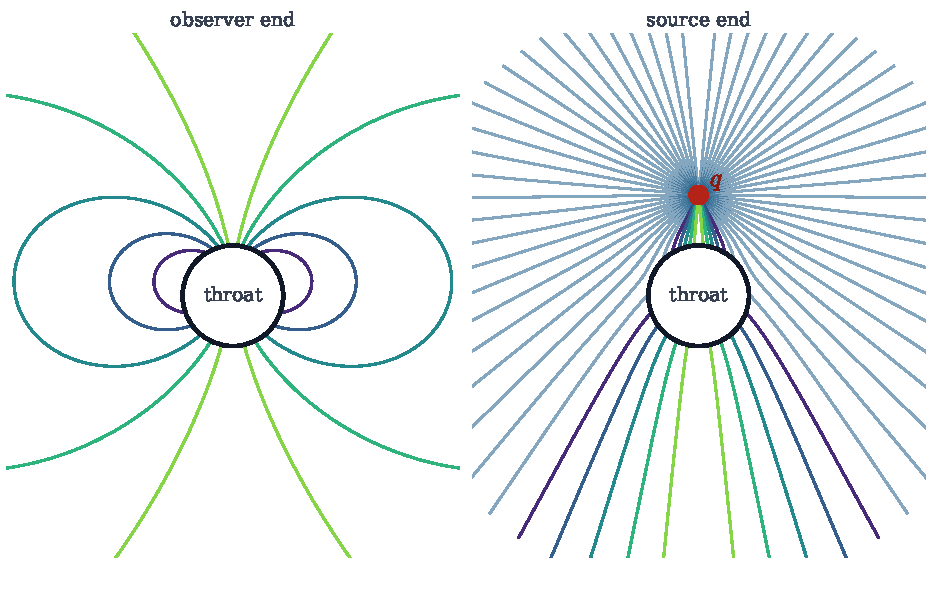
\includegraphics[width=0.82\textwidth]{figures/fig_thinshell_fixed_monopole_flux_v7.pdf}
  \caption{The zero-flux member of Eq.~\eqref{eq:ds-multipoles}: $B_0=0$,
  requiring $c_2-c_1=q/A$.  The black circles represent the same throat sphere
  in the two exterior charts.  Field lines cross the throat but return through
  another angular band, giving zero net flux.  The
  observer-side field is nonzero and contains only $\ell\ge1$ terms.}
  \label{fig:fixed-sector-field}
\end{figure}

\FloatBarrier

\section{Constancy of the first-order mass monopole}
\label{sec:gravity}

In the DS construction the Schwarzschild exteriors have
$d\bar s^2=-f\,dt^2+f^{-1}dr^2+r^2d\Omega^2$, with
$f=1-r_g/r$, and are joined at $R>r_g$.
In their revised preprint, the observer-side static perturbation is
\cite{DaiStojkovic2019ObservingV3}
\begin{equation}
 h^{\mathrm{obs}}_{tt}=\frac{2b}{r_2},\qquad
 h^{\mathrm{obs}}_{rr}=\frac{2br_2}{(r_2-r_g)^2},\qquad
 b=\frac{\mu R}{A}.
 \label{eq:ds-observer-mode}
\end{equation}
Both components give
$h^{\mathrm{obs}}_{\alpha\beta}=b\,\partial_M\bar g_{\alpha\beta}$:
$b$ is a mass shift, with far-field acceleration $-b/r_2^2$, not an
arbitrary potential coefficient.

At first order about Schwarzschild, the harmonic sectors decouple.
The monopole equation therefore applies independently of the source's
nonspherical motion.

\begin{samepage}
Promoting $A$ to $A(t)$ makes this perturbation the linearization of
the metric above with $f$ replaced by
$F(t,r_2)=1-2[M+b(t)]/r_2$.  The linearized mixed Einstein component is
\begin{equation}
 \delta G^r{}_t=\frac{2\dot b}{r_2^2}
 =-\frac{2\mu R\dot A}{A^2r_2^2}.
 \label{eq:momentum-constraint}
\end{equation}
Vacuum therefore requires $\dot b=0$: the proposed monopole modulation
vanishes.  The constant mass shift is fixed by the initial data, not by
the instantaneous orbital radius.
In spherical symmetry, Krasnikov identified this obstruction using
Birkhoff's theorem \cite{Krasnikov2020CommentObserving}.
\end{samepage}

More generally, every vacuum
$\ell=0$ perturbation is a constant mass shift plus a coordinate change
\cite{MartelPoisson2005SchwarzschildPerturbations}.
A time-dependent gauge term cannot supply an observable mass change.
The argument is local to the observer's vacuum region; it assumes
neither vacuum at the throat nor any asymptotic structure.
Higher multipoles remain possible.  Using Sgr~A*/S2 length scales, the
static stiff-shell calculation in Appendix~\ref{app:quadrupole} gives a
quadrupolar acceleration scale of order
$10^{-8}$ times the proposed monopole scale.  Repeated passages could
exceed this estimate if they resonantly excite a weakly damped quadrupolar
mode \cite{CardosoFranzinPani2016Ringdown}.

\section{Nonincrease of the observer-end mass}
\label{sec:nonlinear}

For a two-ended asymptotically flat wormhole, let $E_B(u)$ be the observer
end's Bondi energy: the asymptotic mass monopole in a fixed Bondi frame.
With regular Bondi asymptotics and vacuum near that end's future null
infinity, the standard exact balance law is
\cite{BondiVanderBurgMetzner1962Gravitational,Sachs1962Asymptotic,
WaldZoupas2000Conserved}
\begin{equation}
 E_B(u_2)-E_B(u_1)
 =-\frac{1}{32\pi}\int_{u_1}^{u_2}du
    \int_{S^2}N_{AB}N^{AB}\,d\Omega\le0,
 \qquad u_2>u_1.
 \label{eq:bondi-integrated}
\end{equation}
Here $N_{AB}=\partial_u C_{AB}$ is the Bondi news, with
$g_{AB}=r^2q_{AB}+rC_{AB}+O(1)$, $q^{AB}C_{AB}=0$, and angular indices
raised with the inverse $q^{AB}$ of the unit-sphere metric $q_{AB}$.
Thus $E_B$ cannot rise even if
the source and throat evolve nonlinearly; no energy condition on the
supporting matter is needed.  Applying $A\mapsto A(u)$ to the first-order
DS mode of Eq.~\eqref{eq:ds-observer-mode} would give
$E_B(u)=M+b(u)=M+\mu R/A(u)$.  This rises as the source approaches the
throat and cannot describe the observer-end mass.  Source motion may still
modulate the rate of radiative loss.

When both mouths share one asymptotic region, its Bondi energy belongs
to the whole system, not to either mouth.  At finite separation, coupling
between an external tidal field and the mouth's quadrupole can also
contribute to the mass inferred from orbital motion in the quasistatic
regime \cite[Sec.~I]{Favata2001TidalWork}.  Increasing the exterior
separation suppresses the influence between the mouths through ordinary
space while retaining their connection through the throat.

Suppose a family with exterior
mouth separation $D$ and a fixed source--throat experiment converges
smoothly on every compact spacetime region containing the source, throat,
and corresponding fixed-radius observer-side cuts to a two-ended
spacetime with the above asymptotics.  Let $E_H^{(D)}(u,r)$ be the quasilocal
Hawking energy of such a cut.  Smooth convergence at fixed $r$, followed by
$r\to\infty$ along asymptotically round outgoing cuts, gives the Bondi
energy of the limiting observer end \cite{MarsSoria2015HawkingEnergy}:
\begin{equation}
 \lim_{r\to\infty}\lim_{D\to\infty}E_H^{(D)}(u,r)
 =E_B^{\mathrm{lim}}(u).
 \label{eq:one-ended-limit}
\end{equation}
The limiting observer-end mass is therefore nonincreasing; the argument
gives no finite-separation or finite-radius bound.

\section{Conclusion}
\label{sec:conclusion}

Maxwell charge cannot change without current through the measuring
surface, and the first-order Schwarzschild mass monopole is fixed in
vacuum.  The proposed DS orbital monopole signal comes from treating the
radius dependence of static solutions as an allowed time evolution.
At an observer end that
is vacuum near future null infinity, the exact Bondi law forbids mass
gains.  For mouths sharing one exterior, this result is recovered in an
assumed regular two-ended limit as their separation grows.  Source motion
can still produce higher multipoles and modulate radiative mass loss.

\begin{acknowledgments}
The author thanks Ilia Slobodov for helpful discussions.
\end{acknowledgments}

\section*{Artificial Intelligence Use Statement}

The author used OpenAI ChatGPT/Codex and Anthropic Claude as interactive
assistants for brainstorming, mathematical and editorial critique, prose
revision, consistency checks, reference searches, and figure preparation.  All
arguments, calculations, citations, figures, and conclusions were reviewed and
revised by the author, who is solely responsible for the manuscript.

\appendix
\section{A quasistatic quadrupole benchmark}
\label{app:quadrupole}

We estimate the quasistatic tidal response as the source moves.  At first
order about Schwarzschild, the even-parity $\ell=1$ vacuum mode is a
locally pure-gauge displacement; the odd-parity mode is a constant
angular-momentum shift \cite{MartelPoisson2005SchwarzschildPerturbations}.
The first local, gauge-invariant time-dependent vacuum field is therefore
quadrupolar \cite{Thorne1980Multipole}, unlike the Maxwell dipole in
Fig.~\ref{fig:fixed-sector-field}.

We compare its quasistatic acceleration with the proposed monopole scale
$a_{\mathrm{DS}}\sim\mu R/(Ar_2^2)$.
In the tidal approximation, the quadrupolar part of the source potential
at the throat scales as $\mu R^2/A^3$, and the transmitted potential
decays as $(R/r_2)^3$.
Radial differentiation therefore gives
\begin{equation}
 \frac{a_2}{a_{\mathrm{DS}}}
 \sim C_2\left(\frac{R}{A}\right)^2
          \left(\frac{R}{r_2}\right)^2.
 \label{eq:quadrupole-benchmark}
\end{equation}
To calculate $C_2$, use the static stiff-shell construction of
Ref.~\cite[Appendix~D.1]{CardosoEtAl2017LoveNumbers}.  Its polar metric
amplitudes on the source and observer sides are
$H_0^{(s)}=\alpha P_2^2(x)+\beta Q_2^2(x)$ and
$H_0^{(o)}=\gamma Q_2^2(x)$, where $x=r/M-1$; no applied tide is present
on the observer side.  With the surface-density perturbation set to zero,
the angular metric amplitude $K$ and its derivative along the continuous
tortoise coordinate are continuous at the throat.  Equivalently,
\begin{equation}
 \frac{\gamma}{\alpha}
 =\frac12\left(\frac{K_P}{K_Q}-\frac{K_P'}{K_Q'}\right)_{r=R},
 \qquad
 C_2=\frac85\left(\frac{M}{R}\right)^5\frac{\gamma}{\alpha}.
 \label{eq:quadrupole-transfer}
\end{equation}
Here $K_P,K_Q$ follow from the cited relation between $K$ and $H_0$ by
inserting $P_2^2,Q_2^2$, respectively; primes denote outward $r$ derivatives.
The normalization follows from $P_2^2(x)\sim3x^2$,
$Q_2^2(x)\sim8/(5x^3)$ and the factor three from radial differentiation.
This gives $0<C_2<5/2$ for $R>2M$, approaching $5/2$ in the weak-field
limit and zero as $R\to2M$.

For favorable Sgr~A*/S2 parameters $A\sim R\sim r_g$,
$r_g\simeq0.084\,\mathrm{AU}$ and $r_2\simeq1000\,\mathrm{AU}$,
the geometric factor in Eq.~\eqref{eq:quadrupole-benchmark} is
$7\times10^{-9}$.  With $C_2<5/2$, the quasistatic stiff-shell model
gives $a_2/a_{\mathrm{DS}}\lesssim2\times10^{-8}$.
The near-mouth substitution is an order-of-magnitude extrapolation of
the tidal scaling, not an exact orbital calculation.
We retain $R-r_g\gg\mu$ for perturbative consistency.

\bibliographystyle{apsrev4-2}
\bibliography{references,references_v11_additions}

\end{document}
